%% Standalone figure: compile this file once (pdflatex boundcharge.tex) to produce boundcharge.pdf,
%% which main.tex includes with \includegraphics. Recompile only after editing the figure.
\documentclass[11pt,tikz,border=2pt]{standalone}
\usepackage{amsmath,amssymb}       % \text, \vec, math symbols
\usetikzlibrary{arrows.meta}       % Stealth arrow tips
\begin{document}
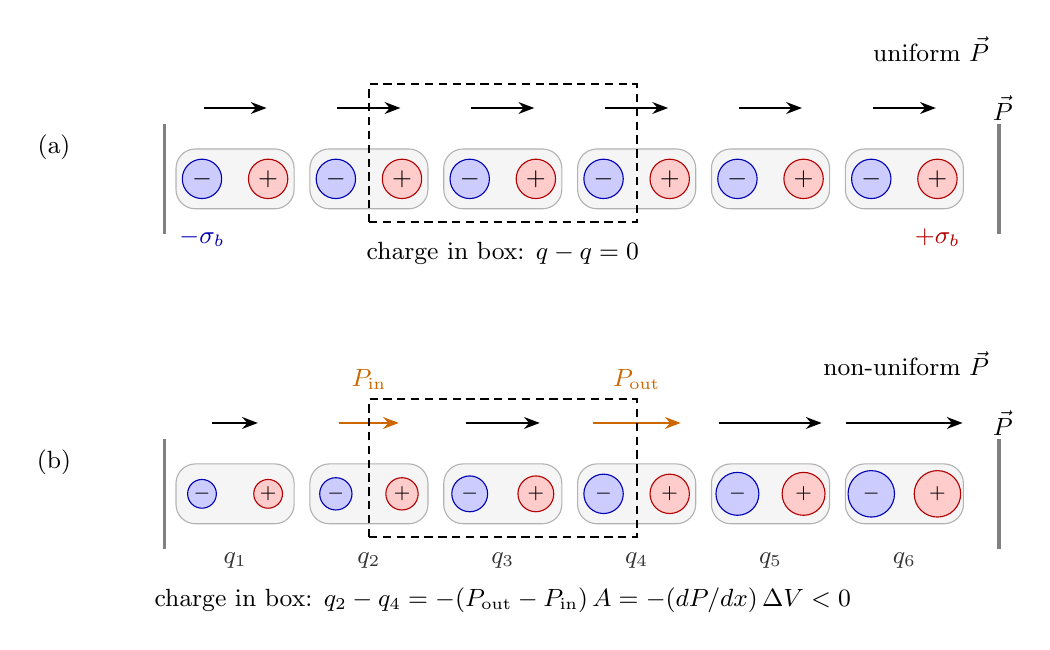
\begin{tikzpicture}[
  font=\small,
  >={Stealth[length=2mm]},
  negcharge/.style={circle, draw=blue!70!black, fill=blue!20, inner sep=0pt},
  poscharge/.style={circle, draw=red!70!black,  fill=red!20,  inner sep=0pt},
  mol/.style={rounded corners=7pt, draw=gray!60, fill=gray!8},
  box/.style={thick, densely dashed},
]
  % ============ (a) uniform polarization ============
  \begin{scope}[yshift=4.0cm]
    \node at (-0.6,0.4) {(a)};
    \node[anchor=east] at (11.4,1.65) {uniform $\vec P$};
    \foreach \k in {1,...,6}{
      \pgfmathsetmacro{\c}{1.7*\k}
      \draw[mol] ({\c-0.75},-0.38) rectangle ({\c+0.75},0.38);
      \node[negcharge, minimum size=5mm] at ({\c-0.42},0) {$-$};
      \node[poscharge, minimum size=5mm] at ({\c+0.42},0) {$+$};
      \draw[->, thick] ({\c-0.4},0.9) -- ({\c+0.4},0.9);
    }
    \node[anchor=west] at (11.2,0.9) {$\vec P$};
    \draw[very thick, gray] (0.8,-0.7) -- (0.8,0.7) (11.4,-0.7) -- (11.4,0.7);
    \node[blue!70!black] at (1.28,-0.75) {$-\sigma_b$};
    \node[red!70!black]  at (10.62,-0.75) {$+\sigma_b$};
    % box from the centre of dipole 2 to the centre of dipole 4
    \draw[box] (3.4,-0.55) rectangle (6.8,1.2);
    \node at (5.1,-0.95) {charge in box: $q - q = 0$};
  \end{scope}

  % ============ (b) non-uniform polarization ============
  \node at (-0.6,0.4) {(b)};
  \node[anchor=east] at (11.4,1.65) {non-uniform $\vec P$};
  \foreach \k in {1,...,6}{
    \pgfmathsetmacro{\c}{1.7*\k}
    \pgfmathsetmacro{\s}{3.2+0.45*\k}      % circle size grows with q_k
    \pgfmathsetmacro{\L}{0.2+0.09*\k}      % arrow half-length grows with P
    \draw[mol] ({\c-0.75},-0.38) rectangle ({\c+0.75},0.38);
    \node[negcharge, minimum size=\s mm] at ({\c-0.42},0) {\scriptsize$-$};
    \node[poscharge, minimum size=\s mm] at ({\c+0.42},0) {\scriptsize$+$};
    \ifnum\k=2 \def\col{orange!80!black}\else\ifnum\k=4 \def\col{orange!80!black}\else\def\col{black}\fi\fi
    \draw[->, thick, \col] ({\c-\L},0.9) -- ({\c+\L},0.9);
    \node[gray!40!black] at (\c,-0.85) {$q_{\k}$};
  }
  \node[anchor=west] at (11.2,0.9) {$\vec P$};
  \draw[very thick, gray] (0.8,-0.7) -- (0.8,0.7) (11.4,-0.7) -- (11.4,0.7);
  % box from the centre of dipole 2 to the centre of dipole 4
  \draw[box] (3.4,-0.55) rectangle (6.8,1.2);
  \node[orange!80!black, anchor=south] at (3.4,1.2) {$P_{\text{in}}$};
  \node[orange!80!black, anchor=south] at (6.8,1.2) {$P_{\text{out}}$};
  \node at (5.1,-1.35) {charge in box: $q_2 - q_4 = -(P_{\text{out}}-P_{\text{in}})\,A = -(dP/dx)\,\Delta V < 0$};
\end{tikzpicture}
\end{document}
